
\marginpar{\href{https://youtu.be/mHfn_7ym6to}{Video}}

Read: 3.1-3.3

\subsection{Continuous Random Variables and PDF's}

Random variables are functions on the sample space.

\begin{figure}[!ht]
\centering
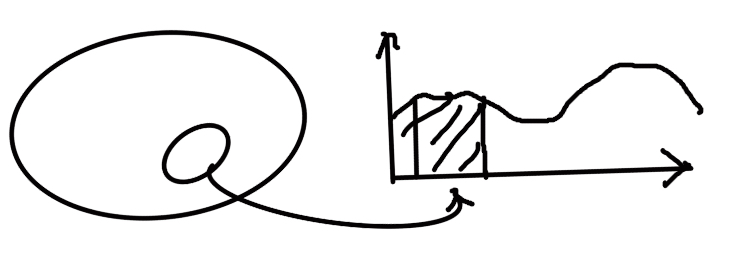
\includegraphics[width=6cm, height=4cm]{images/L08/continuous_rv.jpeg}
\caption{x}
\end{figure}

\begin{align*}
P(a \le X \le b) = \int_a^b f_X(x)dx \\
\int_{-\infty}^\infty f_X(x)dx=1 \\
P(X=a)=0 \\
f_X \ge 0\\
\end{align*}

\subsection{Mean and Variance}

\marginpar{(13:55)}

\begin{align*}
E[X] = \int_{-\infty}^{\infty} x f_X(x)dx
\end{align*}

\begin{align*}
E[g(X)] = \int_{-\infty}^{\infty} g(x) f_X(x)dx
\end{align*}

\begin{align*}
var[X] = \sigma_X^2 = \int_{-\infty}^{\infty} (x - E[X]^2 f_X(x)dx = E[X^2] - (E[X])^2
\end{align*}

\subsection{Continuous Uniform Random Variable}

\marginpar{(13:55)}

\begin{center}
    \begin{tikzpicture}[scale = 0.6]
       \begin{axis}[unit vector ratio=1 1.65 1,
       axis lines = left,
       ymin=-0.0025,ymax=1.2075,xmin=-0.5, xmax = 2.2, 
       % xtick={0,0.5,1,1.5,2,2.5,3},ytick={0.5,1}
       xticklabels={,,},yticklabels={,,}
       ]
       \addplot[very thick,domain=-1:0,blue] {0};
       \addplot[very thick,domain=0:1,blue] {0.5};
       \addplot[very thick,domain=1:2,blue] {0};
       % \addplot[very thick,domain=2:2.5,blue] {1};
       % \addplot[very thick,domain=2.5:3.3,blue] {0};
       \draw[very thick, blue, -] (axis cs:0,0) -- (axis cs:0,0.5);
       \draw[very thick, blue, -] (axis cs:1,0) -- (axis cs:1,0.5);
       % \draw[very thick, blue, -] (axis cs:2,0) -- (axis cs:2,1);
       % \draw[very thick, blue, -] (axis cs:2.5,0) -- (axis cs:2.5,1);
    \end{axis}
\end{tikzpicture}
\end{center}

\begin{figure}[h]
\centering
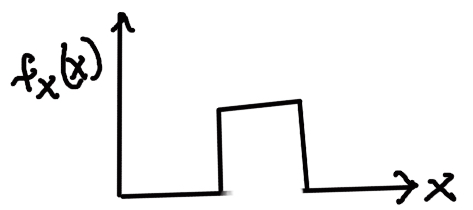
\includegraphics[width=6cm, height=4cm]{images/L08/continuous_unif_pdf.jpeg}
\caption{Continous Uniform Random Variable}
\end{figure}

$h=\frac{1}{b-a}$

Intervals of the same length have the same probability.

\begin{align*}
f_X(x)=\begin{cases}\frac{1}{b-a}, a \le x \le b\\
        0, otherwise
        \end{cases}
\end{align*}

\begin{align*}
E[X] = \int_a^b x\cdot \frac{1}{b-a}dx = \frac{a+b}{2}, \text{midpoint}
\end{align*}

\begin{align*}
\sigma_X^2= = \int_a^b (x - \frac{a+b}{2})^2 = \frac{1}{b-a}dx = \frac{(b-a)^2}{12}\\
\sigma_x = \frac{b-a}{\sqrt{12}}
\end{align*}

\subsection{Cumulative Distribution Function (CDF)}

\marginpar{(20:35)}

Unifying concept of continuous and discrete random variables.

\begin{align*}
F_X(x) = P(X \le x) = \inf_{-\infty}^{\infty} f_X(t)dt
\end{align*}

\begin{figure}[ht]
\centering
\begin{minipage}{.45\linewidth}
  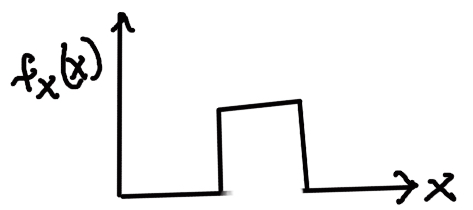
\includegraphics[width=\linewidth]{images/L08/continuous_unif_pdf.jpeg}
  \caption{PMF}
  \label{continuous_unif_pdf}
\end{minipage}
\hspace{.05\linewidth}
\begin{minipage}{.45\linewidth}
  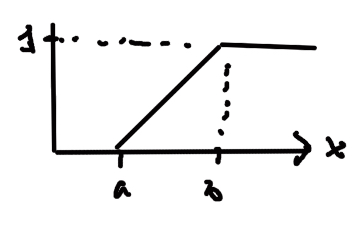
\includegraphics[width=\linewidth]{images/L08/continuous_cdf.jpeg}
  \caption{CDF}
  \label{continuous_cdf}
\end{minipage}
\end{figure}

\edef\mylst{"1/6","3/6","2/6",""}

\begin{figure}[ht]
\centering
\begin{minipage}{.45\linewidth}
  % 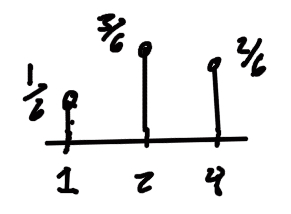
\includegraphics[width=\linewidth]{images/L08/discrete_pmf.jpeg}
\begin{tikzpicture}[scale = 0.7]
\begin{axis} [ymin = 0, ymax = 0.75, xmin = 0, xmax = 4.5,
		y tick label style={
        /pgf/number format/.cd,
            fixed,
            precision=2,
        /tikz/.cd,
        % nodes near coords = {1/6 3/6}
        % nodes near coords
        nodes near coords=\pgfmathsetmacro{\mystring}{{\mylst}[\coordindex]}\mystring,
    }]
\addplot+[ycomb] plot coordinates { (1, 1/6) (2, 3/6) (4, 2/6)}; 
\end{axis}
\end{tikzpicture}
  
  \caption{PMF}
  \label{img1}
\end{minipage}
\hspace{.05\linewidth}
\begin{minipage}{.45\linewidth}
  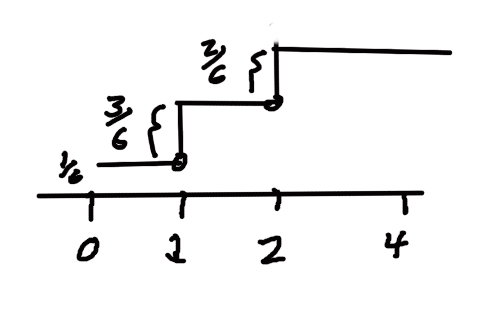
\includegraphics[width=\linewidth]{images/L08/discrete_cdf.jpeg}
  \caption{CDF}
  \label{img2}
\end{minipage}
\end{figure}

\marginpar{(27:40)}

Not all RV's are continuous or discrete.  Can be neither or a mixture of both.

\begin{figure}[h]
\centering
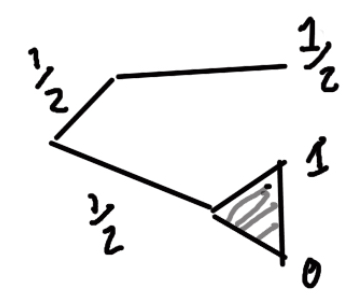
\includegraphics[width=5cm, height=4cm]{images/L08/mixed_rv.jpeg}
\caption{Mixed RV/Mixed Distribution}
\end{figure}

\subsection{Gaussian (Normal) PDF}

\marginpar{(27:40)}

Sum of many small RVs is Normal.

\begin{figure}[h]
\centering
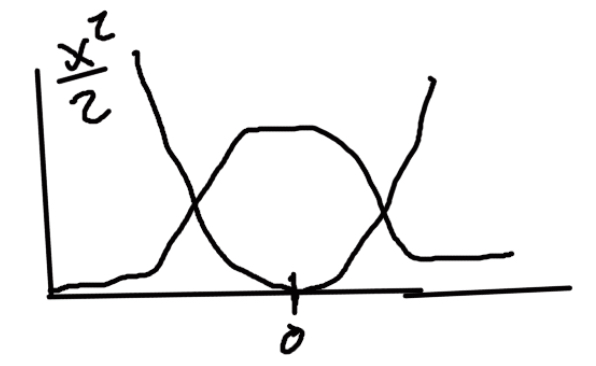
\includegraphics[width=5cm, height=4cm]{images/L08/gaussian_pdf.jpeg}
\caption{x}
\end{figure}

Standard normal $N(0,1)$

\begin{align*}
f_X(x) = \frac{1}{\sqrt{2\pi}} e^{-x/2}
\end{align*}

$\frac{1}{\sqrt{2\pi}}$ is the constant that makes the integral integrate to 1.

Gaussian centered at different places
\begin{align*}
&f_X(x) = \frac{1}{\sigma\sqrt{2\pi}} e^{-(x-\mu)/2\sigma^2}\\
&\mathbb{E}[X]=\mu \\
&var(X)= \sigma^2
\end{align*}

Let $Y=aX+b$
\begin{align*}
&E[Y]=a\mu+b\\
&var(Y)= a^2 \sigma^2\\
&Y \sim N(a\mu+b, a^2 \sigma^2)\\
\end{align*}

\marginpar{(41:30)}

\begin{align*}
\int_{-\infty}^{\bar{x}} e^{-x^2/2}dx
\end{align*}

No closed form solution.  We tabulate it.  There's only a table for standard normal $N(0,1)$.

If $X \sim N(2,16)$:

\begin{align*}
P(X \le 3) = P\left( \frac{X-2}{4} \le \frac{3-2}{4} \right) = CDF(0.25)=0.3987
\end{align*}

If $X \sim N(\mu,\sigma^2)$ then standardize:

\begin{align*}
\frac{X- \mu}{\sigma} \sim N(0,1)
\end{align*}

NOTE: Densities are not probabilities, they are rates at which probabilities accumulate.
